\section{Introduction} \label{sec:introduction}

A fundamental objective of evolutionary biology is to understand how complex phenotypic traits and new genetic information originate.
Among other factors, theory identifies gene duplication as a major contributor to biological complexity \citep{Zhang2003,Otto2000,Wagner2008,Wagner2007,Crow:2006role,Magadum:2013wu,Metz:chromosomeDuplication1947}.
While comparative genomic studies have provided an increasingly detailed account of events shaping genetic and phenotypic traits over natural history \citep{Zhang2014}, substantial ambiguities remain in bridging these findings with explicit, process‑based models of evolutionary dynamics \citep{Welch2016}.
In particular, regarding the contribution of gene duplications to the evolution of complexity, the roles of neo‑functionalization, sub‑functionalization, and dose effects remain active areas of inquiry \citep{Innan2010}.

Within the contemporary field of evolutionary biology, experimental approaches have developed as a key complement to retrospective studies in establishing causality within evolutionary dynamics \citep{Kawecki2012}.
On themes of genetic and functional complexity, in particular, notable contributions complementing \textit{in vivo} work have arisen from studies of digital model systems \citep{Fortuna2022}.
% In this regard, several useful capabilities are unique to \textit{in silico} work.
While considerably lacking in realism and richness compared to biological organisms, \textit{in silico} approaches offer unique capabilities in support for first-principles definitions of complexity, fast throughput spanning upwards of thousands of generations, and flexible exploration of arbitrary counterfactuals.
One particularly notable model system in this vein has been the Avida digital evolution platform, which allows evolution experiments to be conducted using poulations of self-replicating computer programs \citep{Ofria:2009avida}.
Owing to heritable variation introduced through imperfect replication and differential success in self-replicating efficiency, a process of evolution by natural selection unfolds within these populations \citep{pennock2007models}.

A formative early work in this vein, \citet{lenski2003evolutionary} used Avida to investigate the apparent paradox of irreducible complexity.
The primary subject of this study was the EQU trait, a computational task involving a large enough number of constituent substeps that it was nearly never observed to arise spontaneously.
By rewarding resource benefits for completion of simpler tasks, involving fewer substeps, however, the probability of evolving the EQU trait increased profoundly.
Further analysis, enabled by availability of detailed lineage histories, demonstrated that these simpler tasks were serving as building blocks for the more complex EQU task.
Other work has applied Avida to investigate wide-ranging aspects of the evolution of comlexity, investigation the influence of selection on information theoretic measures of complexity \citep{Adami2000Evolution}, how co-evolutionary red queen dynamics can drive the evolution of complex traits \citep{Zaman2014Coevolution}, and how phenotypic complexity relates to abundance within ghe genotype-phenotype map \citep{Fortuna2017GenotypePhenotype}.

Here, we applied digital evolution approaches using Avida to probe the relationship between gene duplication processes and the evolution of complexity.
Mirroring larger questions around the adaptive framings of evolutionary origins of biological complexity, gene duplication is thought to lead to increased complexity both by increasing opportunities for the accumulation of contingent complexity (``sub-functionalization'') and by facilitating adaptive discovery of beneficial novel traits (``neo-functionalization'').
To discern the relevance of novel adaptation in complexity arising from gene duplication, we measured how duplications influenced both phenotypic complexity --- measured in terms of the quantity and composition of rewarded subroutines performed --- and genetic complexity --- measured as the number of genome sites contributing to an organism's fitness.

In a first set of experiments, we looked at how rapidly brittleness accumulated in genomes subject to slip-duplication over their lineage versus those that were simply long to begin with.
We show that brittleness between these two conditions is comparable, contrary to what would be expected under a neutral framing of gene duplication.
However, compatible with a adaptation-based framing of gene duplication, we find evidence that the accumulation of vestigial coding information is accelerated under this condition.
Examining the rate of adaptive evolution, we indeed see that phenotypic traits are gained faster in the presence of slip duplication.
Zeroing in on the character of facilitated traits, we find that this effect is specific to complex traits and that there is not a benefit with respect to simpler traits.
Using a spread of intermediate controls allowing only certain aspects of the effects of slip duplications were enabled, we narrow down this effect specifically to the duplication of genetic information.
Using the capability of the digital model for detailed tracking, we also find that slip duplication of a site increases its subsequent likelihood to code for novel phenotypic traits.
Thus, our findings support the credibility and demonstrate the viability of gene duplications contributing in an adaptation-centric role around the evolution of complexity.

% In our experiment, we used the capabilities of the digital evolution platform to compare evolutionary outcomes in terms of the complexity of traits evolved when mutational processes that duplicated genome regions were included, excluded, as well as a .

% Gene duplication events are widely recognized as a key factor in the evolution of organismal complexity.
% Mirroring broader contrasts between adaptation- versus contingency-driven hypotheses for the evolutionary origins of biological complexity, gene duplication outcomes are typically framed in terms of neo- and sub-functionalization scenarios.
% In the former, duplicated genetic material catalyzes novel functionality; in the latter, it is co-opted to elaborate existing functionality.
% Examples of both scenarios are widespread in natural history, but practical constraints have limited direct experimental investigation of the relationship between gene duplication and organismal complexity.
% Using the Avida platform for digital evolution, we show that while increased genome size can promote the emergence of simple adaptive traits, gene duplication uniquely facilitates the \textit{de novo} evolution of complex adaptive phenotypes.
% Tracing the ancestry of individual genetic sites, we find that slip duplication of a site increases its subsequent likelihood to code for novel phenotypic traits.
% We then harness the unique \textit{in silico} capabilities of our model system to compare evolutionary outcomes across degraded variants of full-fledged gene duplication.
% This ablative analysis confirms that the observed adaptive potentiation indeed arises from the duplication of existing genetic information.
% In contrast to purely neutral framings of biological complexity, our results support gene duplication events as a contributing factor in adaptive origins of complex traits.

% paragraph 3: recap how experiment differentiates between alternate hypotheses, recap major results



% Concrete phenotypic effects have been directly attributed to changes in copy count, such as the short leg length characteristic of dachshunds arising from an additional copy of the FGF4 gene \citep{dachshundGeneCopyNum}.

Duplications in genetic material range from repeats of gene fragments to whole genome duplication.
By providing new genetic material, these events are thought to introduce potential for further evolutionary modification.
As such, duplication is understood to be an essential driver for genetic variation \citep{Zhang:2003fw,Crow:2006role,Magadum:2013wu}.
Indeed, gene duplication has been shown to promote adaptive evolution in both biological and simulation models \citep{Hu:2010ea}.
% [x] AML (2025): I shortened the above definition of evolvability for succintness (folks should make sure they still agree with it). Even better, if we could streamline the sentence to not have a definition interrupt the flow.
% MAM Done; I've been scraping out most discussion of evolvability in favor of just discussion "promotion of adaptive evolution"

% A striking example of gene duplication leading to new adaptations comes from the Long-Term Evolution Experiment in \textit{Escherichia coli}, where a duplication in one population broadened expression of key metabolic machinery to previously inhibitive conditions \citep{blount_genomic_2012}.
% As a result, the population was able to metabolize citrate, a previously inaccessible carbon resource, resulting in a 7-fold increase in population size.

% In addition to such anecdotal case studies, large-scale genomic analyses have discovered cases where a strikingly high fraction of the genes in an organism show evidence of having arisen from gene duplications \citep{teichmann_structural_1998,Teichmann:2004cz}.
% Comparative studies have associated duplication events early in natural history with increases in genetic robustness and evolutionary innovation \citep{wagner_gene_2008}.

% The prominent role of gene duplications in biological evolution has inspired incorporation of analogous mechanisms in evolution-inspired optimization algorithms \citep{Ryan:1998gm,Sawai:1999genetic,Sawai:2000comparative,Schmitt:2005bc}.
% Notably, in genetic programming, gene duplication and deletion operators have been shown to increase program evolvability and yield simpler evolved solutions \citep{Koza:1995fr}.
% In work evolving neural controllers for robots, enabling module duplication was found to increase functional specialization in network modules \citep{Calabretta:1998vh,Calabretta:2000tl}.

Given the evidence that gene duplication can facilitate adaptive evolution in both computational and natural systems, we use a digital evolution approach to explore \textit{why}.
That is, what mechanistic aspects of gene duplications promote adaptive evolution?

One question is how fidelity of duplicated material influences subsequent evolutionary outcomes.
Exact duplications can result in functionally redundant genes that can increase the mutational robustness of a genotype \citep{Crow:2006role} or allow the organism to produce additional gene product \citep{Zhang:2003fw}.
If a highly constrained genetic sequence is duplicated, one copy can potentially mutate more freely and produce new functionality (i.e., neofunctionalization) \citep{Zhang:2003fw,Wagner:2003fk}.
Alternatively, subfunctionalization may occur where both gene copies diverge from the ancestral gene state, specializing in complementary aspects of the ancestral gene's functionality \citep{Zhang:2003fw}.

It is also possible that ``side effects'' of gene duplication may contribute to adaptive evolution, such as effects in increasing effective mutation rate, localized clustering of sequence changes, and increases in genome length.
Due to their inherent co-occurrence, it is not obvious how to disentangle these aspects of gene duplication in field or laboratory studies.


In our experiments, we implemented a series of mutation operators to systematically isolate aspects of gene duplication and tease apart which factors promote evolvability.
Specifically, we use gene duplication mutation operators in Avida that resemble replication slippage \citep{bzymek_instability_2001} (\textit{slip mutations}) and allow for gene duplications or deletions at any scale.
When slip mutations were present, we found that the populations evolved complex tasks significantly faster.
Moreover, by analyzing the dominant lineage of each population, we observed that complex tasks, when first evolved, were signficantly more likely to depend on instructions within duplicated regions of the genome.
Together, these results strongly suggest that gene duplication plays a pivotal role in the evolution of traits with multiple components, providing insight into the origin of intricate natural systems.

\begin{figure}[!ht]
\centering
% https://docs.google.com/presentation/d/109vfeK_lHSsE0q7Iz7tzl9sDxnP8jyOF2gJ-v85pgL8/edit?usp=sharing
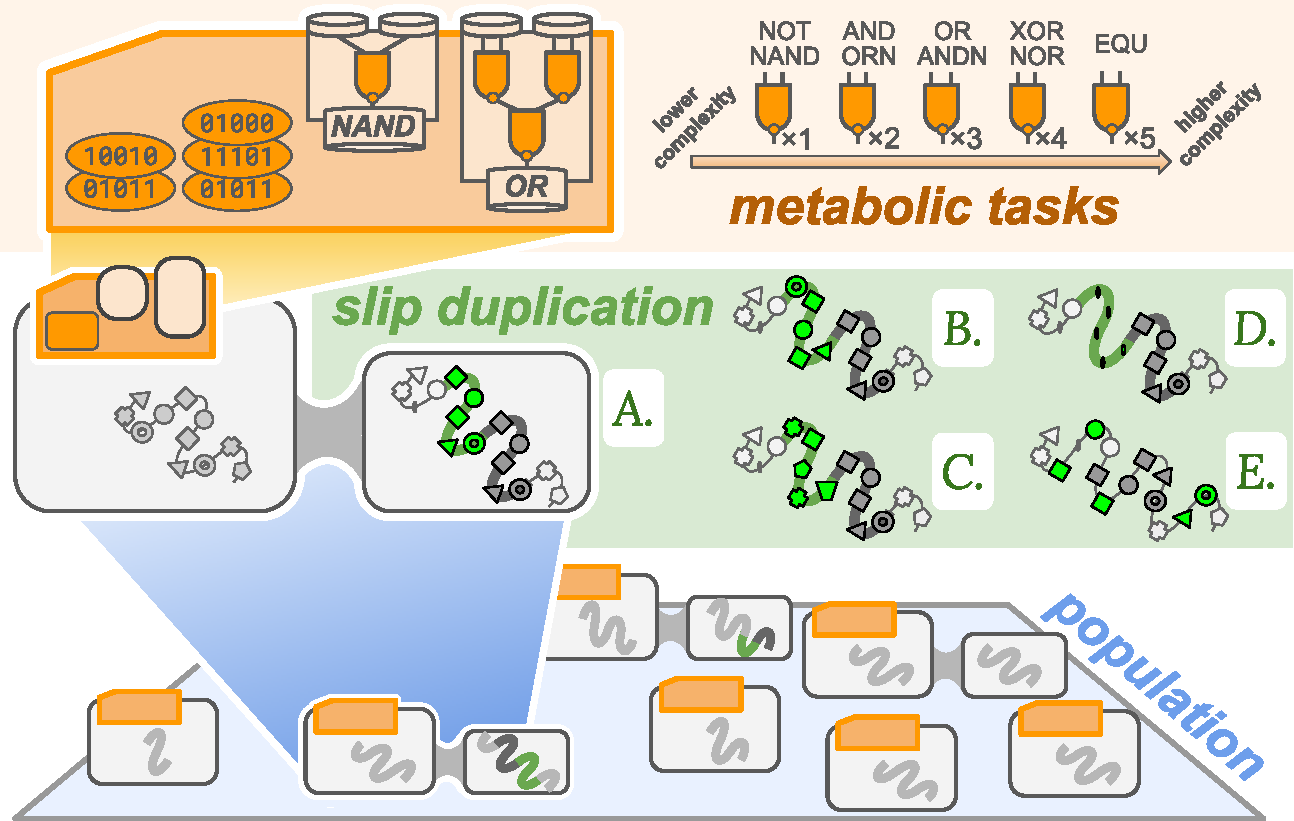
\includegraphics[width=\linewidth]{imgs/GeneDupeOps.pdf}

\vspace{2ex}

\caption{%
\textbf{Genome replication and phenotypic traits in Avida.}
\footnotesize
Self-replicating computer programs serve as digital model organisms (bottom panel).
Organisms comprise virtual stacks and registers used to store binary values and pointers within a genome of program instructions used to track instruction execution and copying.
Competition to survive and reproduce occurs within a limited-capacity population.
Replication activity can be accelerated by carrying out available ``metabolic'' input/output tasks (top panel).
These tasks vary in complexity with respect to the number of NAND operations required to perform them.
An organism's metabolic ``phenotype'' arises from the expression of its genetic code.
Genetic code copied from parent to offspring may be subject to point mutations, which change the individual instruction values, and slip mutations, which introduce or remove many instructions all at once (slip inserts shown as bright green).
Reported experiments compare five alternate variants of slip mutation:
A) \textit{Slip-duplicate}, an exact duplication is inserted adjacent to the target segment;
B) \textit{Slip-scramble}, shuffled duplication is inserted directly after the target segment;
C) \textit{Slip-random}, random instructions are inserted directly after the target segment;
D) \textit{Slip-NOP}, neutral nop-X instructions are inserted directly after the target segment; and
E) \textit{Slip-scatter}, randomly-drawn instructions are inserted at random throughout the genome.
}
\label{fig:slip_mut_variants}
\end{figure}


FROM COMPARATOR
Figure 1 shows a schematic overview of the relationships between
hosts, functions, resources, and parasites in our experiments. Hosts
obtain the resources necessary for their reproduction by performing
one or more logic functions, but those functions also make the host
vulnerable to infection by a parasite that can perform the same
function. Thus, an infection can occur only if a particular host and
parasite share at least one function, although the specific genetic
encoding that a host and parasite employ to perform that function
rarely, if ever, correspond at the sequence level. After a successful
infection, the parasite acquires 80\% of the infected host’s CPU
cycles, which the parasite uses to execute and copy its own genome,
while imposing a severe cost on the host. As a consequence,
coevolution occurs when hosts and parasites acquire and lose
functions.

FROM COMPARATOR
The experimental configuration allowed for nine different logic
functions, which require varying numbers of NAND instructions
to be executed with the proper inputs used for each; NAND is the
only logic function available in the genetic instruction set. Although
there are many potential measures of functional complexity, the
Avida logic environment provides an intuitive metric, as follows.
The minimum number of NAND operations required for each
function’s performance is known and provides a simple, objective
measure of the complexity of that function [14]. The most complex
function, EQU, requires five NAND operations, and the shortest
program that can perform EQU requires nearly 20 precisely
interacting instructions, although there are many longer programs
that also encode EQU [14]. In the absence of parasites, a previous
study found that 23 of 50 populations evolved the ability to perform
EQU when the other eight functions were rewarded with additional
CPU cycles that increased with their complexity (i.e., minimum required NANDs), thus allowing essential building blocks to
accumulate in the evolving genomes [14]. Here, we test whether
host-parasite coevolution can drive increased complexity without
explicitly rewarding building blocks. To that end, we ran similar
experiments except with coevolving parasites in one-half of the
replicates and without the progressive reward structure used in the
previous work.

% \subsection{Major Results}

% We found local slip mutations that duplicate intact regions to be the most effective configuration of gene duplication in facilitating evolution on the Logic-9 task set within the Avida platform.
% In particular, we found that --- compared to control experiments with long genome sizes --- gene duplication uniquely promoted the evolution of complex adaptive traits.
% We further found that the raw material created by slip duplication plays a potentiating role in the evolution of complex traits.
% Specifically, we identified that slip-duplicated regions are significantly more likely to serve as coding sites for new traits when they first appear.
% Consistent with expectations under neofunctionalization theory, however, we did not observe potentiation effects of slip duplication on the evolution of simple traits, only traits that were facilitated by multiple building block components.

% % [x] @CAO: Since I'm making a lot of changes, I'll start duplicating and commenting out the original text.  I hear that such duplications can accelerate the adaptive process.  ;-)
% Finally, we assessed the consequences of slip duplication on genome architecture.
% One hypothesis is that gene duplication would promote genetic brittleness by increasing genome length and accelerating growth in contingent complexity, as newly redundant genetic material specializes over time.
% % [x] @CAO Do we need to define "genome complexity" before we use it here?
% % @MAM Perhaps we can say something a little more specific instead of "genome complexity"
% Contrary to this possibility, we found that active coding sites grew as a rate similar to control experiments.
% However, we observed that slip duplications produced a significant increase in the accumulation of coding material, when active and vestigial sites are considered together.
% To understand this phenomenon, we tested the immediate effects of slip duplication on genome brittleness.
% We found that, on average, fitness-neutral slip duplications decreased, rather than increased, the number of information-baring sites in a genome.
% These results align with our observed increase in vestigial coding material in genomes.
% These brittleness-reducing effects appear to be counteracted by other factors, resulting in a similar overall trajectory of genome information content between the slip-duplication and control treatments.
